% Bagian Lampiran
\section*{Lampiran} % Jika ada lampiran

% ini buat percobaan 1

\begin{figure}[H]
  \centering
  % Kalau mau menambah gambar lagi tinggal nambahin begin{subfigure} -> end{subfigure}
  \begin{subfigure}[c]{0.4\linewidth}
    \centering
    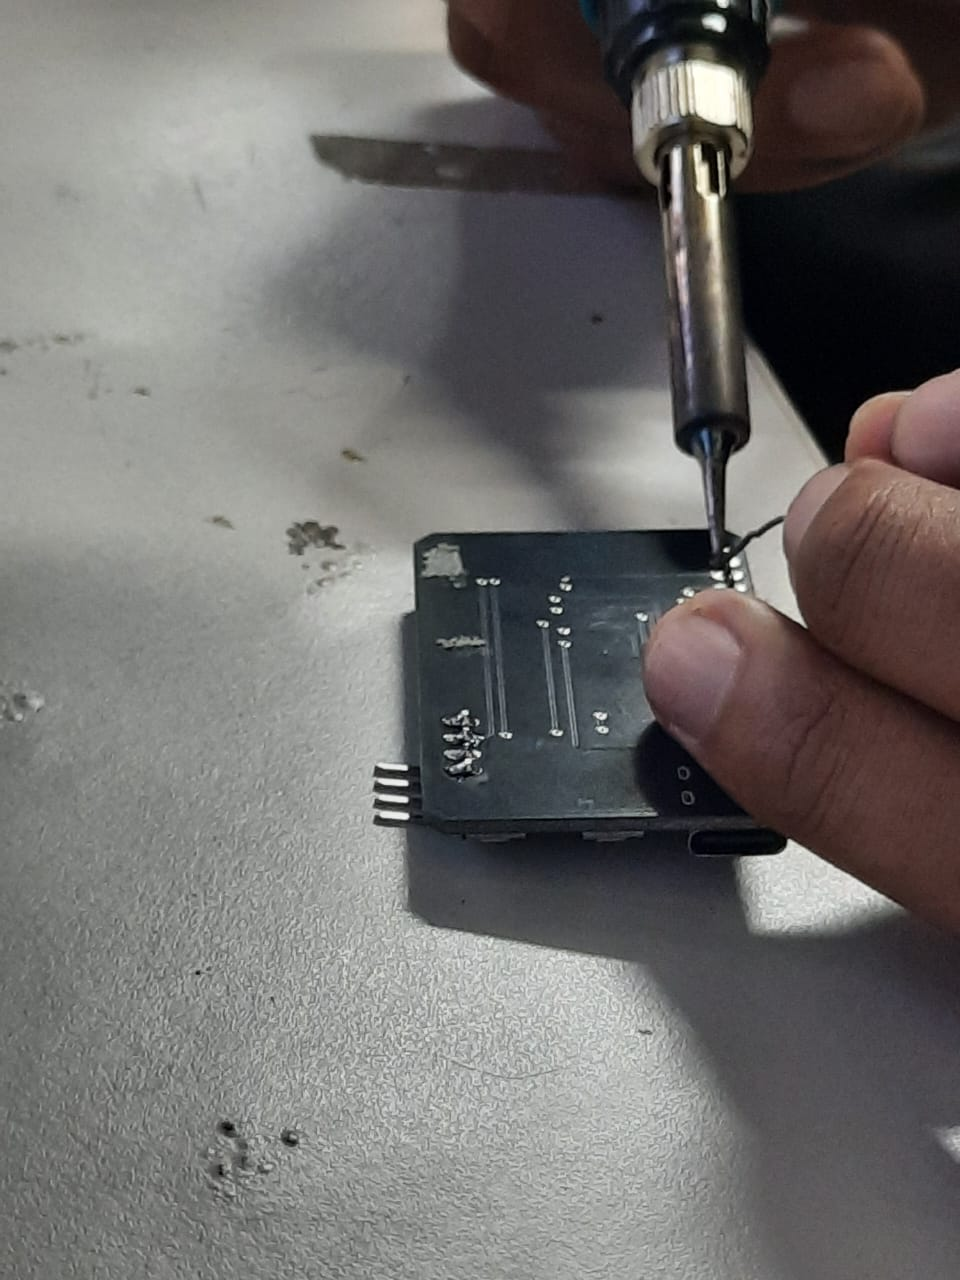
\includegraphics[width=\linewidth]{img/modul_4/proses solder pcb.jpg}
    \caption{Proses peletakan komponen dan soldering PCB\label{fig:inisub1}}
  \end{subfigure}
  \hspace{1cm}
  \begin{subfigure}[c]{0.4\linewidth}
    \centering
    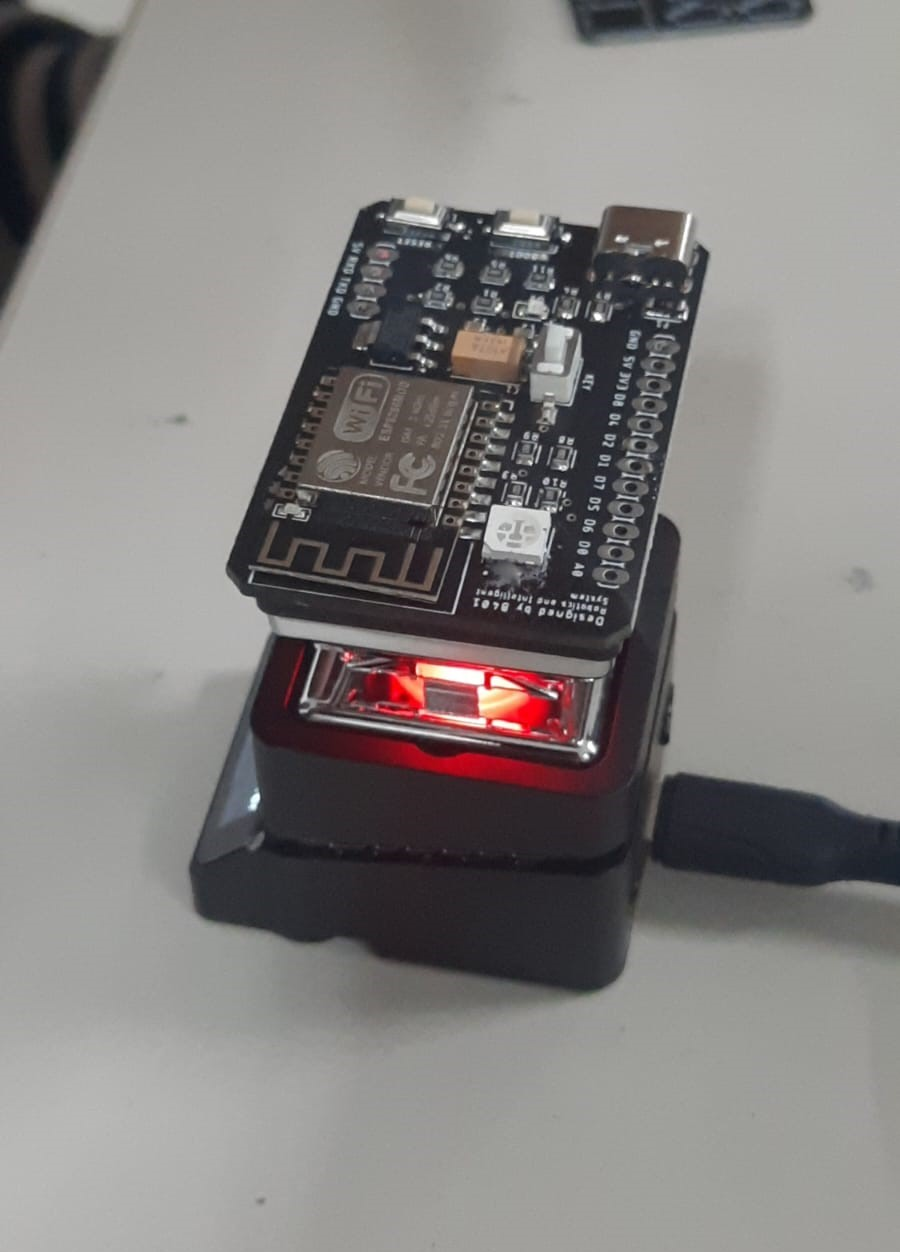
\includegraphics[width=\linewidth]{img/modul_4/proses_pemanasan_pcb.jpg}
    \caption{Proses pemanasan PCB \label{fig:inisub2}}
  \end{subfigure}
  \caption{Proses percobaan \label{fig:keduagambar}}
\end{figure}

\begin{figure}[H]
  \centering
  % Kalau mau menambah gambar lagi tinggal nambahin begin{subfigure} -> end{subfigure}
  \begin{subfigure}[c]{0.4\linewidth}
    \centering
    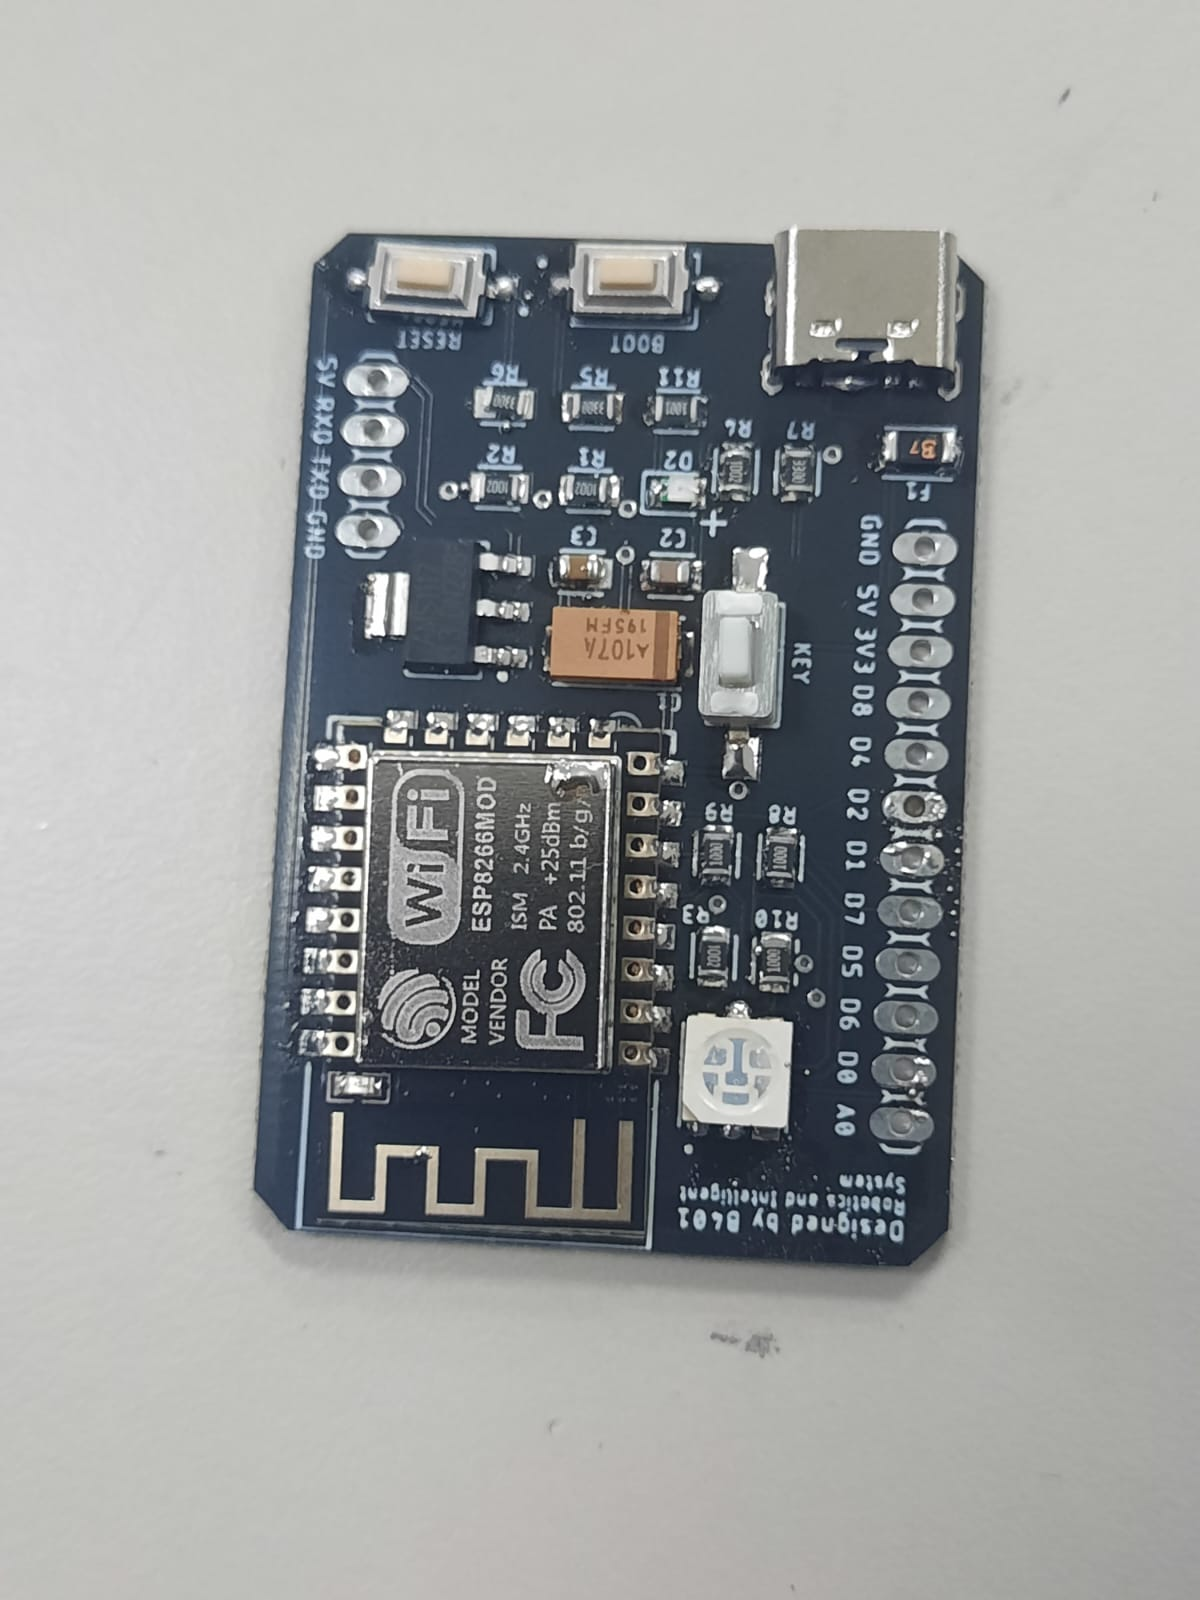
\includegraphics[width=\linewidth]{img/modul_4/hasil_pcb.jpg}
    \caption{Hasil PCB \label{fig:inisub1}}
  \end{subfigure}
  \hspace{1cm}
  \begin{subfigure}[c]{0.4\linewidth}
    \centering
    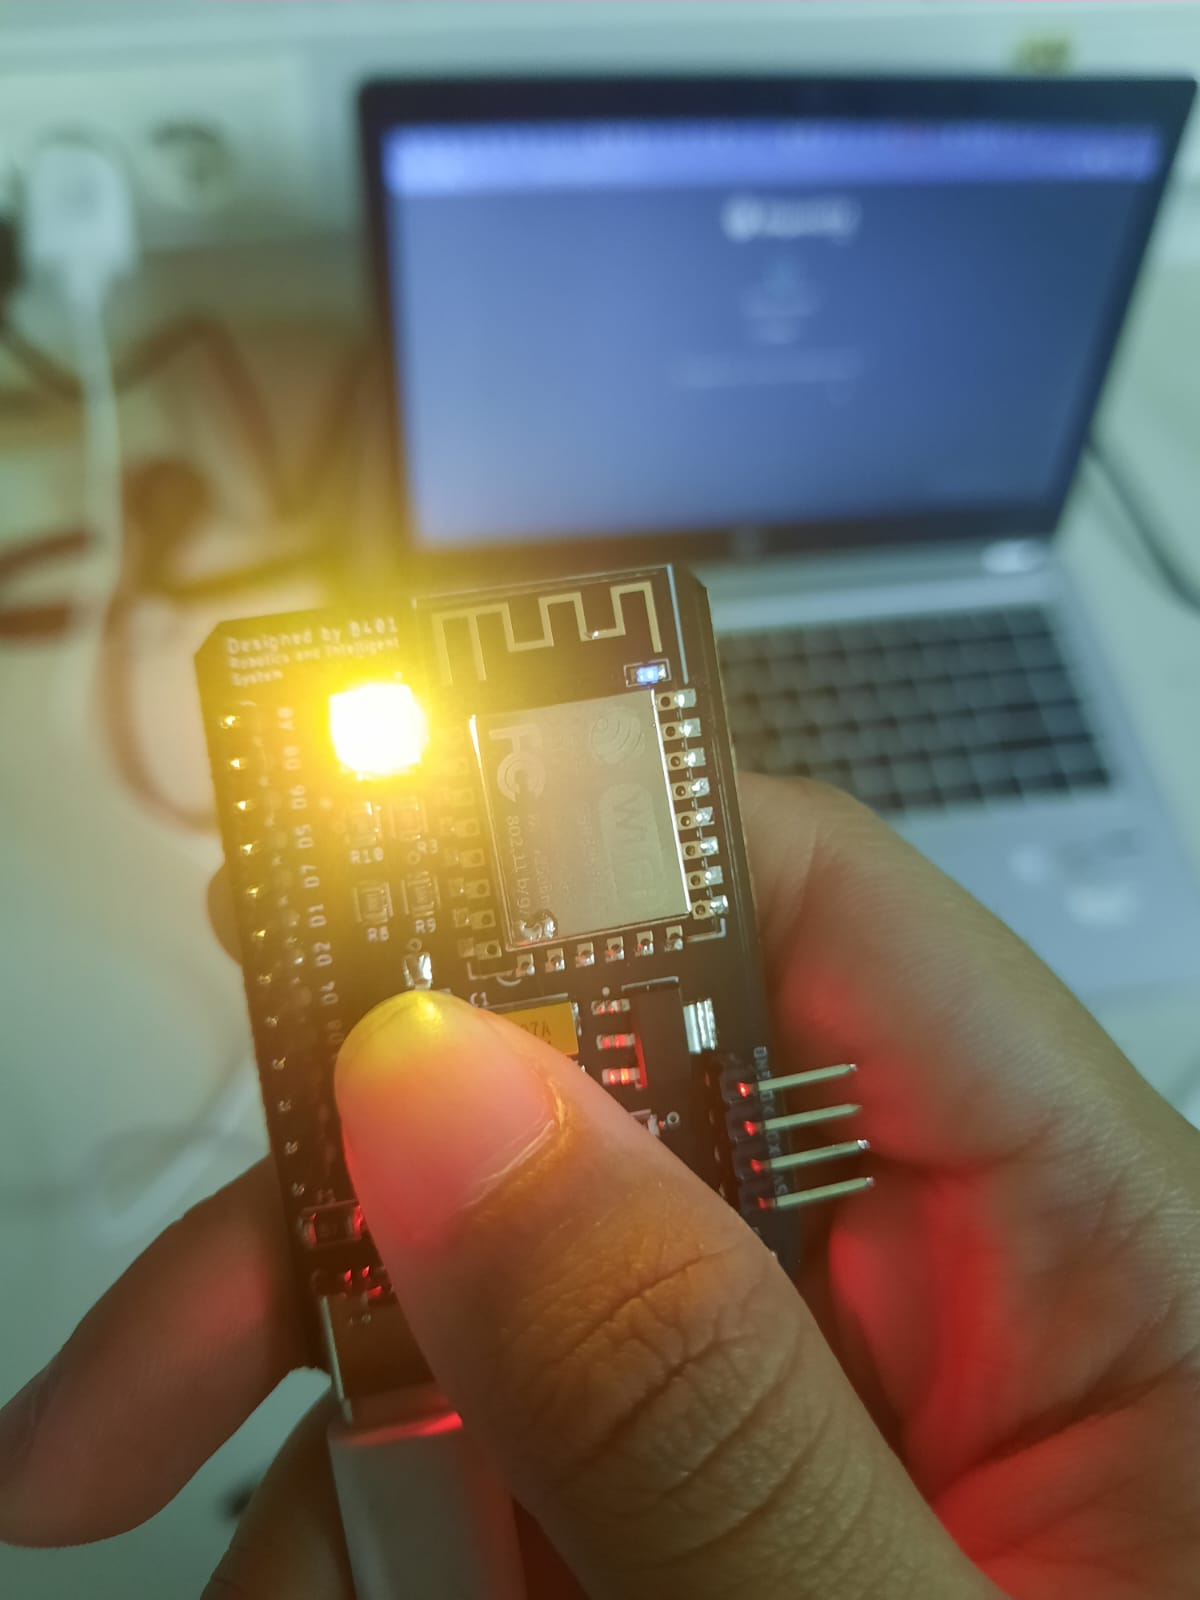
\includegraphics[width=\linewidth]{img/modul_4/hasil_nyala.jpg}
    \caption{Hasil saat LED menyala (button ditekan)\label{fig:inisub2}}
  \end{subfigure}
  \caption*{Hasil percobaan \label{fig:keduagambar}}
\end{figure}